\section{Introduction}
\subsection{ANN}

\begin{frame}
	
	\begin{block}{ANN - Approximate Nearest Neighbors}
		In this brief report, we investigate fast nearest neighbors algorithms (in particular, the library called FLANN). FLANN includes such algorithms as {\color{red} \textit{k-d forest}} and {\color{red} \textit{priority search $k$-means tree}} \cite{Muja2009}. 
	\end{block}
	
	\begin{block}{Notes on Implementation}
		Experiments were performed in Python 3.8.1, using the PyFLANN library. Technical details are available on our  \href{https://github.com/salisaresama/computer-vision/blob/flann-32k/flann.ipynb}{{\color{blue} \underline{GitHub}}} repository.
	\end{block}
	
\end{frame}


\section{Experiments}
\subsection{Description and Notation (1)}

\begin{frame}
	
	\begin{block}{What did we do?}
		\begin{enumerate}
			\item In the scope of this work, naive implementation of the $k$-means \cite{Lloyd1982} clustering algorithm was performed by means of assigning points to clusters using various techniques for nearest neighbors search (see \href{https://github.com/salisaresama/computer-vision/blob/flann-32k/pylib/ann/cluster.py}{{\color{blue} \underline{the respective GitHub page}}}):
			\begin{itemize}
				\item k-d forest;
				\item priority search $k$-means tree;
				\item exact assignment.
			\end{itemize}
			
			\item Clusters were always initialized the same way: randomized initialization by sampling from the uniform distribution $U(\alpha, \beta)$ with constant seed where $\alpha$ and $\beta$ are given by values in the data set (minimum and maximum, respectively).\footnotemark No normalization was involved.
			
			\item Afterwards, we tested the functionality of our implementation on synthetic data (see Fig.~\ref{fig:km_example}) and also its ability to label points for a SIFT data set with approx. 2M records.
		\end{enumerate}	

	\end{block}	

	\footnotetext{\tiny This is only one of many solutions - more optimal ones are available, e.g. $k$-means++ \cite{Arthur2007}.}
	
\end{frame}

\subsection{Description and Notation (2)}

\begin{frame}
	
	\begin{figure}
		\centering
		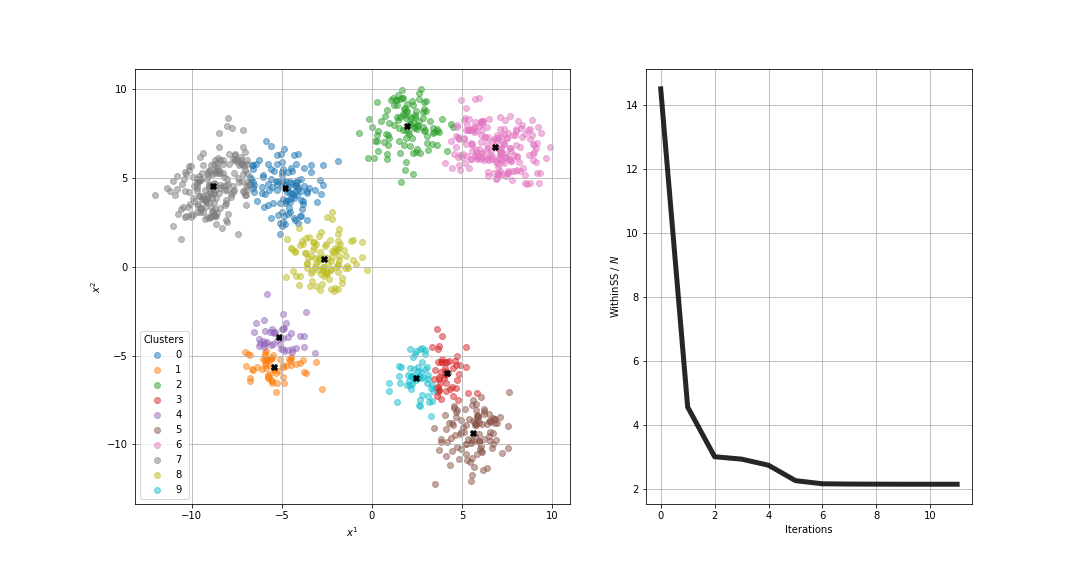
\includegraphics[width=1.0\linewidth]{../images/flann/kmeans_test}
		\caption{\footnotesize Naive $k$-means implementation output with points labeled using the priority search $k$-means tree algorithm.}
		\label{fig:km_example}
	\end{figure}
	
\end{frame}

\subsection{Description and Notation (3)}

\begin{frame}
	
	
	\begin{block}{Framework of Experiments}
		
		\begin{itemize}
			
			\item 	For each NN technique applied on the SIFT data set, we calculate time spent on computations per iteration and visually compare behavior of the cost function $C=$ WithinSS$/ N = \frac{1}{N}\sum_{i = 1}^{N} \lVert X_{i} - f(X_{i})\rVert_{2}^{2}$. The number of cluster centers was set to 32000; each run continued for 30 iterations.
			
			\item \textbf{Notation}:
			
			\begin{itemize}
				\item[-] $X \in \mathbb{R}^{N \times d}$ where $N$ is the number of samples and $d$ is the dimension (in our case, $N = 2097152$, $d = 128$);
				\item[-] $X_{i}$, $i \in \{1, 2, \dots, N\}$, is the $i$-th row of matrix $X$;
				\item[-] $f(X_{i})$ denotes the coordinates of the cluster center associated with $X_{i}$;
				\item[-] $\lVert \cdot \rVert_{2}$ is the Euclidean norm $\left( \lVert \cdot \rVert_{2} = \sqrt{\left< \cdot, \cdot \right>} \right)$.
			\end{itemize}	
		\end{itemize}
		
	\end{block}
	
\end{frame}


\subsection{Runs and Timings (1)}

\begin{frame}
	\begin{block}{Runs}
		Due to bounded computational capabilities, we tested two sets of parameters for approximate nearest neighbors techniques and measured time to evaluate NN and time to assign new cluster centers within individual iterations:
		
		\begin{itemize}
			\item k-d forest ($T$ - number of randomized trees, $C$ - number of leaves to check in one search):
			\begin{table}
				\scriptsize
				\begin{tabular}{| c || c | c | c | c |}
					\hline
					ID & T & C & (AVG. | STD.) NN time, [s] & (AVG. | STD.) assignment time, [s] \\
					\hline
					\hline			
					1 & 32 & 75 & 197.11 | 16.8 & 225.1 | 15 \\
					2 & 64 & 100 & 323.39 | 32.35 & 212.65 | 21.76 \\
					\hline  
				\end{tabular}
			\end{table}
			\item Priority search $k$-means tree ($B$ - branching factor for $k$-means tree construction, $I$ - number of iterations for the tree construction, $CB$ - cluster boundary index for the search in the tree, $C$ - number of leaves to check in one search):
			\begin{table}
				\scriptsize
				\begin{tabular}{| c || c | c | c | c | c | c |}
					\hline
					ID & B & I & CB & C & (AVG. | STD.) NN time, [s] & (AVG. | STD.) assignment time, [s] \\
					\hline
					\hline			
					1 & 32 & 20 & 0.2 & 75 & 102.2 | 39 & 220.6 | 7.29 \\
					2 & 64 & 20 & 0.2 & 100 & 137.07 | 22.14 & 236.47 | 13.22 \\
					\hline  
				\end{tabular}
			\end{table}
		\end{itemize}
	\end{block}
\end{frame}

\subsection{Runs and Timings (2)}

\begin{frame}
	
	\begin{block}{Exact Point Assignment}
		
		\begin{itemize}
			\item With $N \approx 2$M, $d = 128$, and the number of cluster centers equal to 32000, the problem is infeasible for short time frames.
			
			\item We tried to assign points directly by evaluation of distances to all cluster centers and soon halted the calculation, as $\frac{1}{4}$ of the first iteration took approx. 4 hours (30 iterations would result in approx. 20 days).
			
			\item Another tested approach was assignment of points to respective centers by means of standard k-d trees:
			
			\begin{table}
				\scriptsize
				\begin{tabular}{| c | c |}
					\hline
					(AVG. | STD.) NN time, [s] & (AVG. | STD.) assignment time, [s] \\
					\hline
					\hline			
					9085.98 | 4160.11 & 202.04 | 14.03 \\
					\hline  
				\end{tabular}
			\end{table}
			
			\item For the sake of being able to provide at least some margin for comparison of results, we have also performed mini-batch $k$-means clustering \cite{Sculley2010} with same initial cluster centers. It took the algorithm from 6 to 8 hours to converge in 890 iterations. The resulting value of the cost function is equal to 55864.63 (for more information, visit \href{https://github.com/salisaresama/computer-vision/blob/flann-32k/_aux/kmeans_std.ipynb}{{\color{blue} \underline{here}}}).
		\end{itemize}
		
	\end{block}

\end{frame}


\subsection{Results}

\begin{frame}
	
	\begin{figure}
		\centering
		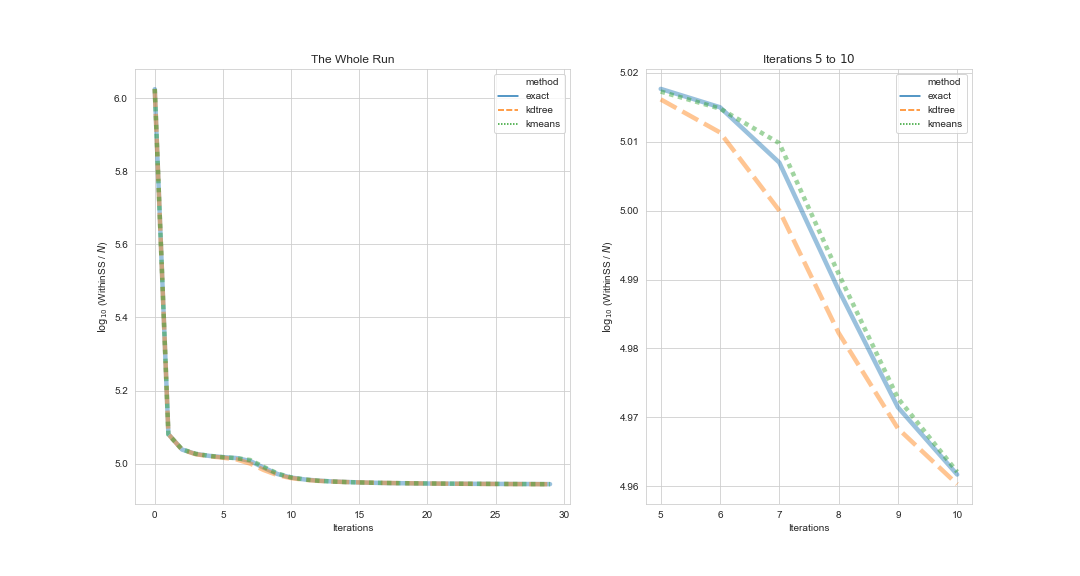
\includegraphics[width=1.0\linewidth]{../images/flann/comparison}
		\caption{\footnotesize Comparison of different approximate nearest neighbors evaluation approaches in the scope of $k$-means iterations.\footnotemark}
		\label{fig:comparison}
		
		\footnotetext{\tiny On the left-hand-side, the priority search $k$-means tree approach stops at iteration 16 due to the fact that the cost function stopped decreasing and no progress was made during the following 10 iterations.}
	\end{figure}
	
\end{frame}


\subsection{Discussion of Results}

\begin{frame}
	The experiment on the previous slide leads to the following conclusions:
	
	\begin{itemize}
		\item For the given set of parameters and data set, the priority search $k$-means tree is faster than the k-d forest for the cost of being less accurate. Nonetheless, its accuracy is comparable to that of a k-d forest approach.
		\item Convergence of ANN-based methods is highly dependent on initial parameters and poor parameter choice might prevent them from progress towards the optimal solution. Examples from Fig.~\ref{fig:comparison} show that convergence of the $k$-means method might be faster with ANN search than that with exact assignment.
	\end{itemize}
	
	Even though the convergence of $k$-means might be faster with ANN assignment during first iterations due to shuffling of poorly labeled points, the cost function is no longer guaranteed to be optimized (see Fig.~\ref{fig:comparison_fix}). The guarantee vanishes by cause of the fact that labels are no longer optimal before cluster centers rearrangement. To prevent the cost function from increasing, we introduce simple post-processing of ANN-based labels:
	
	\begin{itemize}
		\item[-] For points whose new labels are different from that of the previous iteration, we check if their newly assigned centers are indeed closer than the previous ones. If not, old labels are retained. 
	\end{itemize}
\end{frame}


\subsection{Post-Processing Applied}

\begin{frame}
	
	\begin{figure}
		\centering
		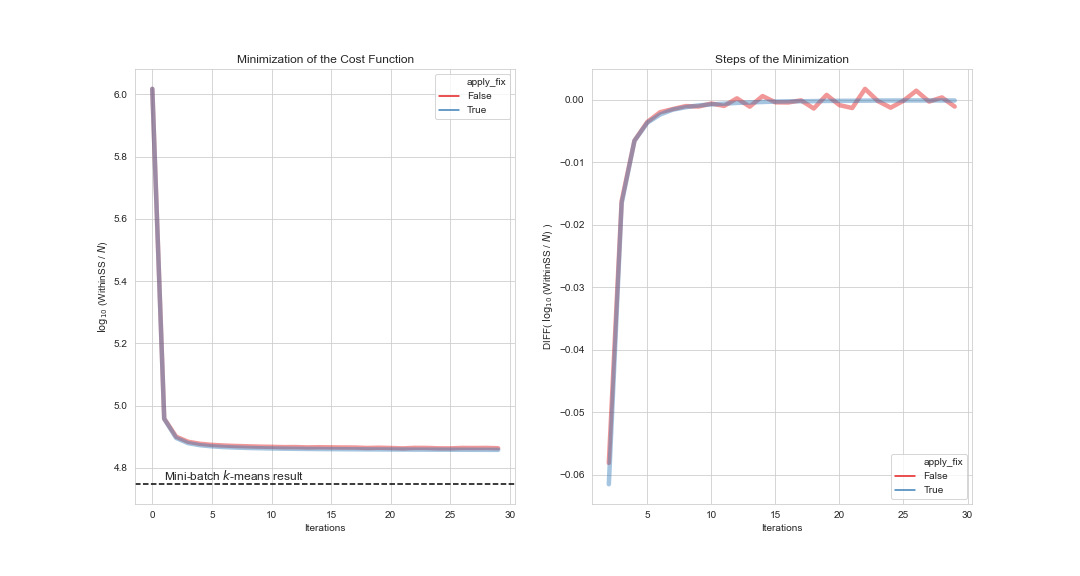
\includegraphics[width=0.975\linewidth]{../images/flann/comparison_fix}
		\caption{
			\scriptsize Performance of the priority search $k$-means tree with and without the proposed post-processing of labels. The diagram confirms that the cost function can increase when the ANN-based label assignment is used. Moreover, it shows that the proposed post-processing procedure fixes the problem. Used parameters:			
			{\tiny
				\centering
				\begin{tabular}{| c || c | c | c | c | c |}
					\hline
					Fix & B & I & CB & C & (AVG. | STD.) NN time, [s] \\
					\hline
					\hline			
					False & 8 & 10 & 0.2 & 25 & 63.06 | 11.1 \\
					True & 8 & 10 & 0.2 & 25 & 63.51 | 8.61 \\
					\hline  
				\end{tabular}
		}}
		\label{fig:comparison_fix}
	\end{figure}

\end{frame}